% =========================================================
% CHAPTER 9: DATABASE DESIGN
% =========================================================
\chapter{Database Design}
\label{chap:database_design}

\section{Database Architecture Overview}
The persistence layer of FraudShield AI is implemented using relational database technologies managed through \textbf{SQLAlchemy 2.0 ORM} and \textbf{Flask-Migrate (Alembic)}. The schema is engineered to guarantee strict referential integrity, atomic financial operations, idempotent migrations, and auditability.

\section{Entity Relationship Diagram (ERD)}
Figure~\ref{fig:erd_diagram} depicts the core relational entities, cardinalities, primary keys, and foreign key relationships.

\begin{figure}[htbp]
    \centering
    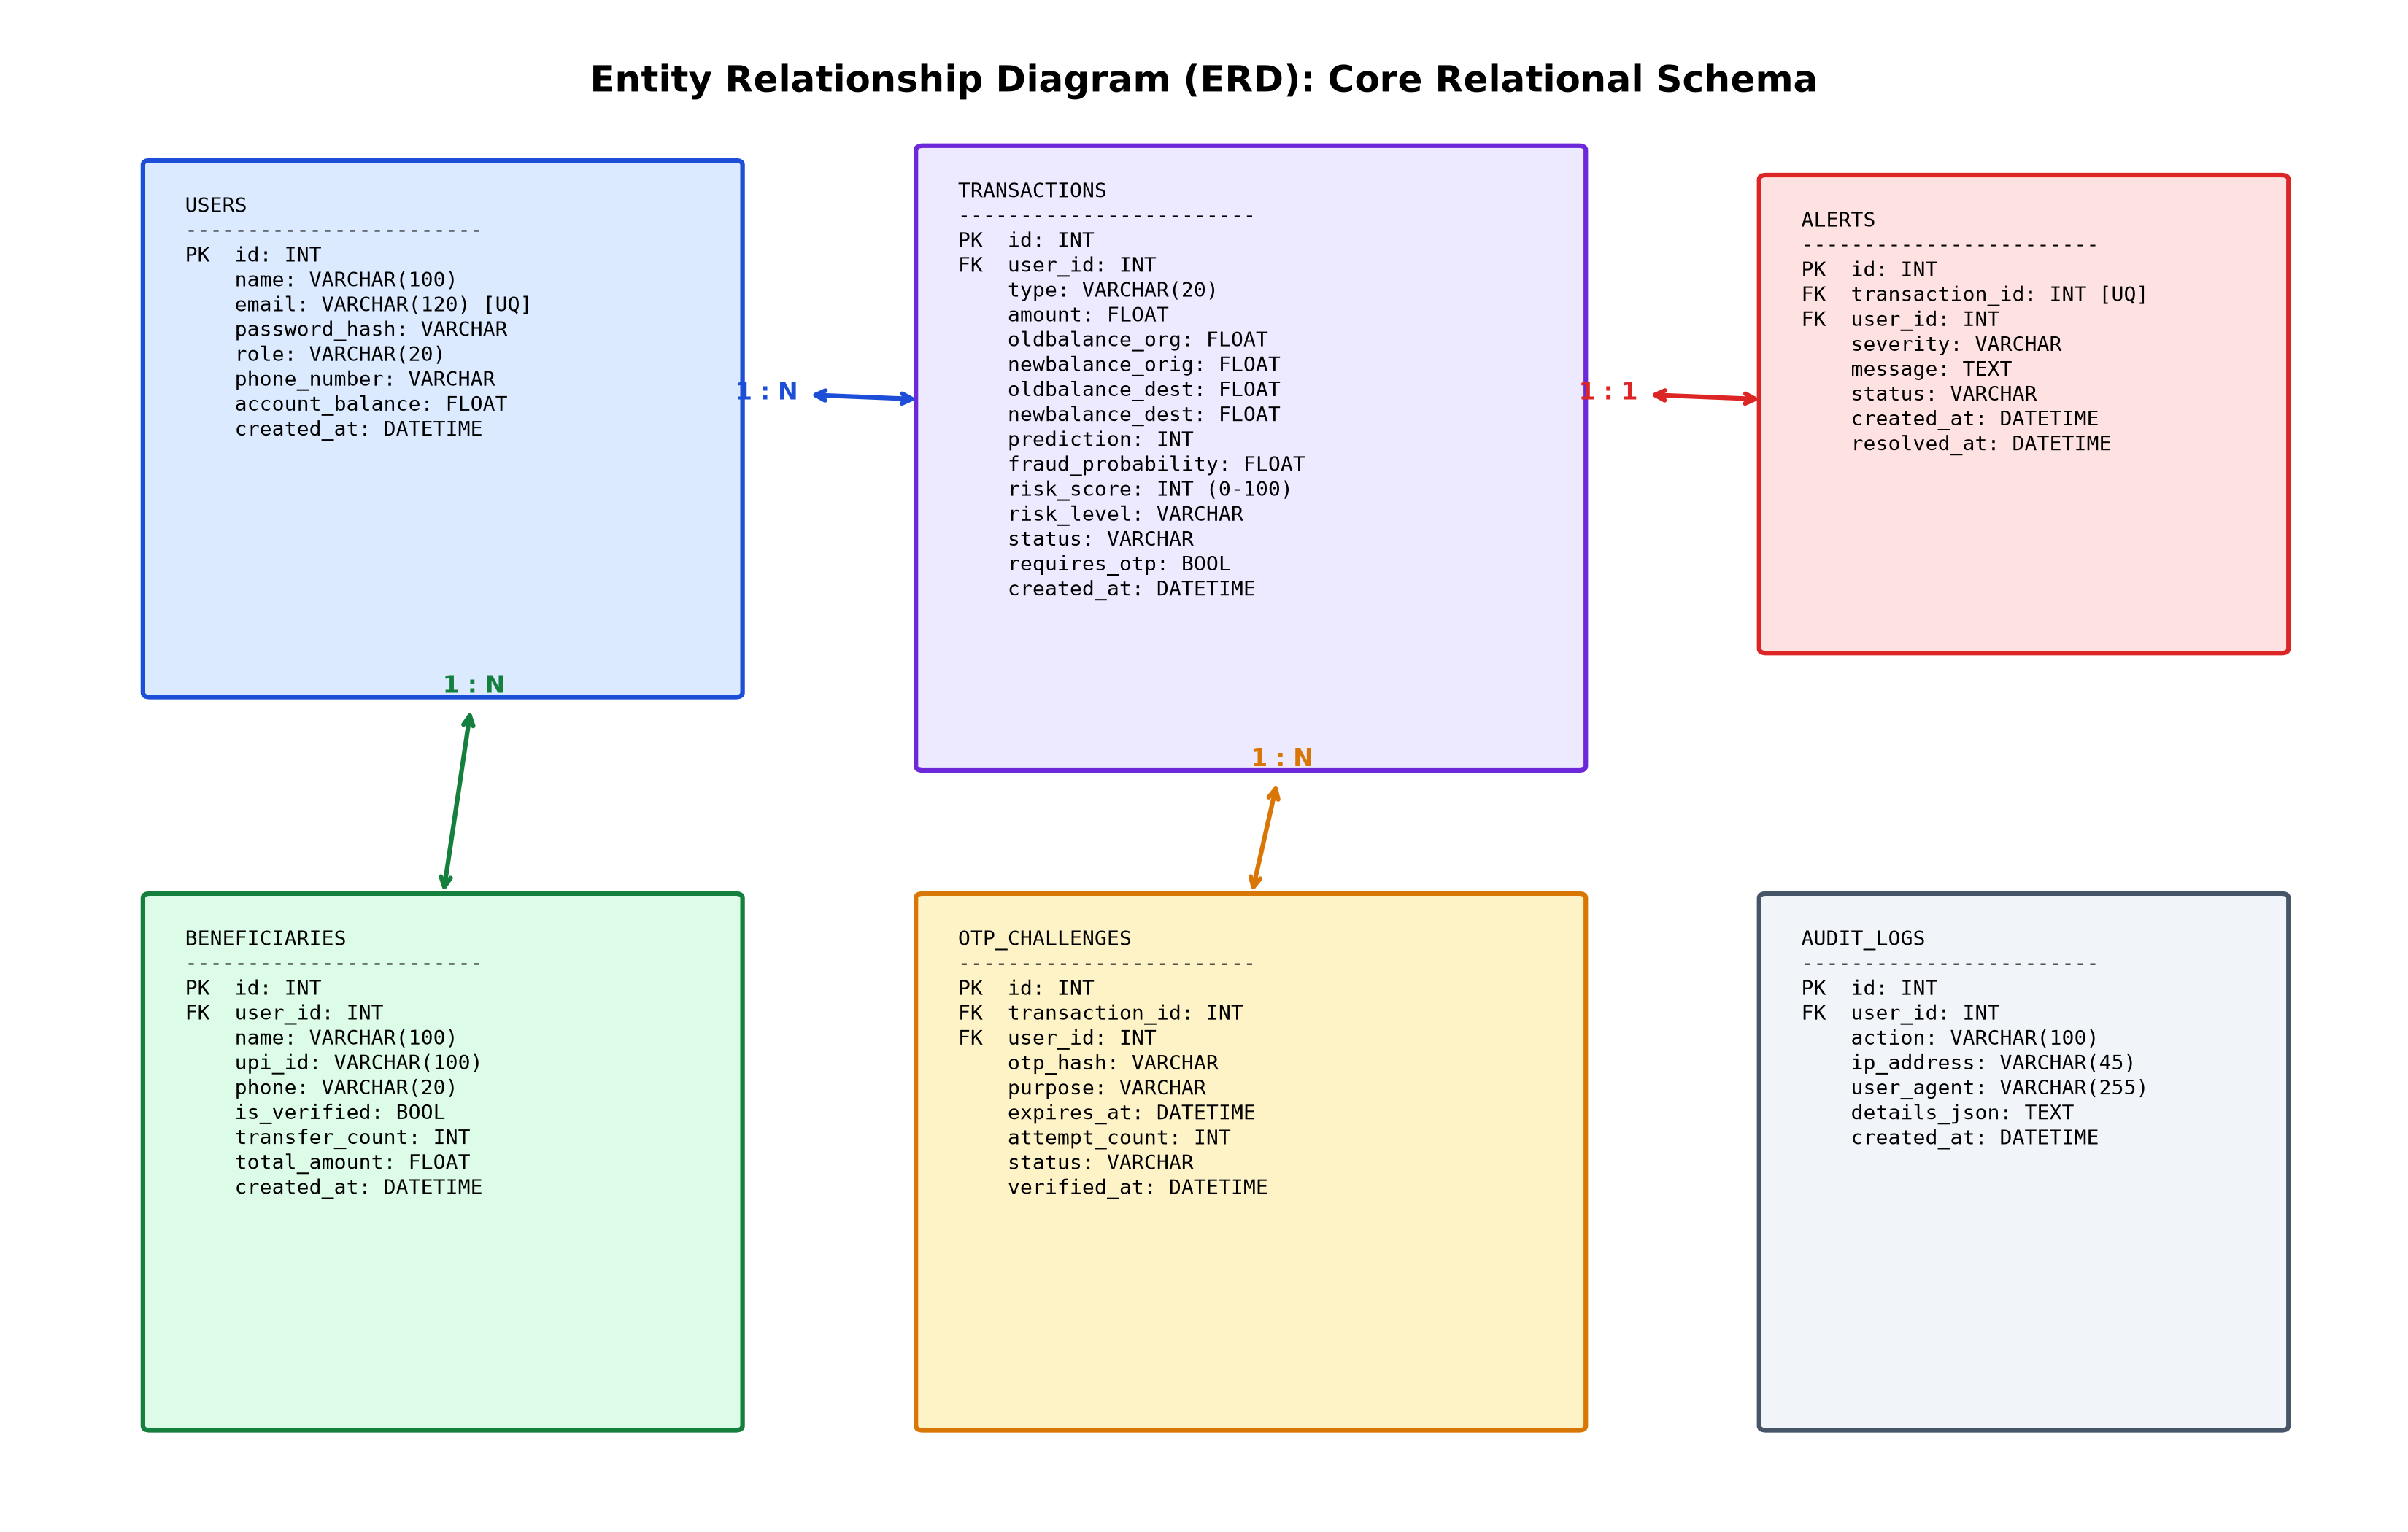
\includegraphics[width=0.92\textwidth]{figures/erd_diagram.png}
    \caption{Entity Relationship Diagram (ERD) of Core Relational Schema}
    \label{fig:erd_diagram}
\end{figure}

\section{Detailed Table Schemas and Constraints}

\subsection{1. \texttt{users} Table}
Stores customer and administrator identities, cryptographic credentials, VPA mappings, and account balances.

\begin{table}[h]
\centering
\caption{Database Schema: \texttt{users} Table}
\label{tab:users_schema}
\begin{tabularx}{\textwidth}{lp{2.8cm}p{1.8cm}X}
\toprule
\textbf{Column Name} & \textbf{Data Type} & \textbf{Nullable} & \textbf{Constraints \& Description} \\
\midrule
\texttt{id} & \texttt{INTEGER} & No & Primary Key, Auto Increment. \\
\texttt{name} & \texttt{VARCHAR(100)} & No & Full customer name. \\
\texttt{email} & \texttt{VARCHAR(120)} & No & Unique, Indexed (\texttt{ix\_users\_email}). \\
\texttt{password\_hash} & \texttt{VARCHAR(255)} & No & Salted PBKDF2/Scrypt hash. \\
\texttt{role} & \texttt{VARCHAR(20)} & No & Check: \texttt{USER} or \texttt{ADMIN}. \\
\texttt{pin\_hash} & \texttt{VARCHAR(255)} & Yes & Salted 4--6 digit numeric PIN hash. \\
\texttt{account\_balance} & \texttt{FLOAT} & No & Default: 100000.0, Check: $\ge 0.0$. \\
\texttt{primary\_upi\_id} & \texttt{VARCHAR(100)} & Yes & Virtual Payment Address (\texttt{user@fraudshield}). \\
\texttt{is\_phone\_verified} & \texttt{BOOLEAN} & No & Default: False. \\
\texttt{created\_at} & \texttt{DATETIME} & No & Indexed account creation timestamp. \\
\bottomrule
\end{tabularx}
\end{table}

\subsection{2. \texttt{transactions} Table}
Maintains the complete financial transaction ledger, ML predictions, risk scores, and serialized SHAP audit payloads.

\begin{table}[h]
\centering
\caption{Database Schema: \texttt{transactions} Table}
\label{tab:transactions_schema}
\begin{tabularx}{\textwidth}{lp{2.8cm}p{1.8cm}X}
\toprule
\textbf{Column Name} & \textbf{Data Type} & \textbf{Nullable} & \textbf{Constraints \& Description} \\
\midrule
\texttt{id} & \texttt{INTEGER} & No & Primary Key, Auto Increment. \\
\texttt{user\_id} & \texttt{INTEGER} & No & Foreign Key $\to$ \texttt{users.id} (On Delete Cascade). \\
\texttt{type} & \texttt{VARCHAR(20)} & No & Payment type (\texttt{TRANSFER}, \texttt{PAYMENT}, etc.). \\
\texttt{amount} & \texttt{FLOAT} & No & Check: \texttt{amount > 0}. \\
\texttt{oldbalance\_org} & \texttt{FLOAT} & No & Sender initial balance prior to transfer. \\
\texttt{newbalance\_orig} & \texttt{FLOAT} & No & Sender final balance after transfer. \\
\texttt{oldbalance\_dest}& \texttt{FLOAT} & No & Recipient initial balance. \\
\texttt{newbalance\_dest}& \texttt{FLOAT} & No & Recipient final balance. \\
\texttt{prediction} & \texttt{INTEGER} & No & Binary ML prediction ($0$ or $1$), Indexed. \\
\texttt{fraud\_probability}& \texttt{FLOAT} & No & Continuous probability $P(\text{fraud}) \in [0.0, 1.0]$. \\
\texttt{risk\_score} & \texttt{INTEGER} & No & Standardized risk score ($0-100$), Indexed. \\
\texttt{risk\_level} & \texttt{VARCHAR(20)} & No & Check: \texttt{LOW}, \texttt{MEDIUM}, \texttt{HIGH}, \texttt{CRITICAL}. \\
\texttt{status} & \texttt{VARCHAR(30)} & No & Status: \texttt{APPROVED}, \texttt{OTP\_REQUIRED}, \texttt{UNDER\_REVIEW}. \\
\texttt{requires\_otp} & \texttt{BOOLEAN} & No & Multi-factor challenge requirement flag. \\
\texttt{explanation\_json}& \texttt{TEXT} & Yes & JSON-serialized SHAP feature attributions. \\
\texttt{created\_at} & \texttt{DATETIME} & No & Compound Index (\texttt{user\_id}, \texttt{created\_at}). \\
\bottomrule
\end{tabularx}
\end{table}

\subsection{3. \texttt{alerts} Table}
Maintains high-priority security incident records generated automatically for SOC investigation.

\begin{table}[h]
\centering
\caption{Database Schema: \texttt{alerts} Table}
\label{tab:alerts_schema}
\begin{tabularx}{\textwidth}{lp{2.8cm}p{1.8cm}X}
\toprule
\textbf{Column Name} & \textbf{Data Type} & \textbf{Nullable} & \textbf{Constraints \& Description} \\
\midrule
\texttt{id} & \texttt{INTEGER} & No & Primary Key, Auto Increment. \\
\texttt{transaction\_id} & \texttt{INTEGER} & No & Foreign Key $\to$ \texttt{transactions.id} (Unique). \\
\texttt{user\_id} & \texttt{INTEGER} & No & Foreign Key $\to$ \texttt{users.id} (On Delete Cascade). \\
\texttt{severity} & \texttt{VARCHAR(20)} & No & Check: \texttt{MEDIUM}, \texttt{HIGH}, \texttt{CRITICAL}. \\
\texttt{message} & \texttt{TEXT} & No & Grounded explanation narrative. \\
\texttt{status} & \texttt{VARCHAR(20)} & No & Check: \texttt{OPEN}, \texttt{RESOLVED}, \texttt{DISMISSED}. \\
\texttt{created\_at} & \texttt{DATETIME} & No & Incident generation timestamp. \\
\texttt{resolved\_at} & \texttt{DATETIME} & Yes & Resolution timestamp. \\
\bottomrule
\end{tabularx}
\end{table}

\subsection{4. \texttt{otp\_challenges} Table}
Stores hashed one-time verification tokens, expiration timestamps, attempt counters, and verification state.

\begin{table}[h]
\centering
\caption{Database Schema: \texttt{otp\_challenges} Table}
\label{tab:otp_challenges_schema}
\begin{tabularx}{\textwidth}{lp{2.8cm}p{1.8cm}X}
\toprule
\textbf{Column Name} & \textbf{Data Type} & \textbf{Nullable} & \textbf{Constraints \& Description} \\
\midrule
\texttt{id} & \texttt{INTEGER} & No & Primary Key, Auto Increment. \\
\texttt{transaction\_id} & \texttt{INTEGER} & No & Foreign Key $\to$ \texttt{transactions.id}. \\
\texttt{user\_id} & \texttt{INTEGER} & No & Foreign Key $\to$ \texttt{users.id}. \\
\texttt{otp\_hash} & \texttt{VARCHAR(255)} & No & Salted PBKDF2 hash of 6-digit OTP code. \\
\texttt{expires\_at} & \texttt{DATETIME} & No & Expiration timestamp (180-second TTL). \\
\texttt{attempt\_count} & \texttt{INTEGER} & No & Default: 0, Max allowed: 3. \\
\texttt{status} & \texttt{VARCHAR(20)} & No & Check: \texttt{ACTIVE}, \texttt{VERIFIED}, \texttt{EXPIRED}, \texttt{EXHAUSTED}. \\
\texttt{verified\_at} & \texttt{DATETIME} & Yes & Successful verification timestamp. \\
\bottomrule
\end{tabularx}
\end{table}

\section{Essential SQL Query Patterns}
\subsection{Atomic Settlement Execution (Double-Debit Protection)}
\begin{lstlisting}[language=SQL, caption={Atomic Settlement and Balance Deduction Query}]
BEGIN TRANSACTION;
-- 1. Deduct amount from sender account
UPDATE users 
SET account_balance = account_balance - :tx_amount 
WHERE id = :sender_id AND account_balance >= :tx_amount;

-- 2. Update transaction status to SETTLED
UPDATE transactions 
SET status = 'APPROVED', decision = 'SETTLED_AFTER_OTP' 
WHERE id = :tx_id AND status = 'OTP_REQUIRED';

-- 3. Mark OTP challenge as verified
UPDATE otp_challenges 
SET status = 'VERIFIED', verified_at = CURRENT_TIMESTAMP 
WHERE id = :challenge_id AND status = 'ACTIVE';
COMMIT;
\end{lstlisting}

\subsection{SOC Incident Triage Query}
\begin{lstlisting}[language=SQL, caption={SOC Open High-Risk Alerts Retrieval Query}]
SELECT a.id, a.severity, a.message, t.amount, t.risk_score, u.email, a.created_at
FROM alerts a
JOIN transactions t ON a.transaction_id = t.id
JOIN users u ON a.user_id = u.id
WHERE a.status = 'OPEN'
ORDER BY t.risk_score DESC, a.created_at DESC;
\end{lstlisting}
